\documentclass[main.tex]{subfiles}
\begin{document}



\section{Topologie in $\mathbb{R}$}
\label{sec:topologie-mathbbr}

\begin{de}
  We noemen een deelzverzameling $A$ van $\mathbb{R}$ \term{open} als het volgende geldt:
  \[ \forall x\in A: \exists \delta \in \mathbb{R}_{0}^{+}, \forall y\in \mathbb{R}:\ |y-x| < \delta \Rightarrow y\in A \]
\end{de}

\begin{st}
  Een $A$ van $\mathbb{R}$ is open als en slechts als het volgende geldt:
  \[ \forall x\in A:\ \exists \delta \in \mathbb{R}_{0}^{+}:\ ]x-\delta,x+\delta[ \subseteq A \]

  \extra{bewijs}
\end{st}

\begin{de}
  Een deelverzameling $B$ van $\mathbb{R}$ noemen we \term{gesloten} als het complement ervan (in $\mathbb{R}$) open is.
\end{de}

\begin{opm}
  ``open'' en ``gesloten'' zijn geen complementaire begrippen.
\end{opm}

\begin{st}
  Open intervallen zijn inderdaad open deelverzamelingen.

  \begin{proof}
    Voor een willekeurige $x$ in een open interval $]a,b[$, vinden we $\delta = min\{x-a,b-x\}$.
    Er geldt dan $]x-\delta,x+\delta[ \subseteq ]a,b[$:
    \[ \forall y\in ]x-\delta,x+\delta[:\ y > x-\delta \ge x-(x-a) = a \ \wedge\ y < x+\delta \le x+(b-x) = b \]
  \end{proof}
\end{st}

\begin{st}
  Open intervallen zijn niet gesloten
  \extra{bewijs}
\end{st}

\begin{st}
  Gesloten intervallen zijn inderdaad gesloten deelverzamelingen.

  \begin{proof}
    Zij $[a,b]$ een gesloten interval.
    We bewijzen dat $X = \mathbb{R} \setminus [a,b] = ]-\infty,a[ \cup]b,+\infty[$ open is.
    Kies daartoe een willekeurige $x\in X$.
    We onderscheiden twee gevallen:
    \begin{itemize}
    \item $x \in ]-\infty,a[$: $0 < \delta \le a-x$
    \item $x \in  ]b,+\infty[$: $0 < \delta \le x-b$
    \end{itemize}
    In beide gevallen geldt $]x-\delta, x+\delta[ \subseteq X$. $X$ is dus open en $[a,b]$ daarom gesloten.
  \end{proof}
\end{st}

\begin{st}
  Gesloten intervallen zijn niet open.
  \extra{bewijs}
\end{st}

\begin{st}
  Halfopen intervallen zijn noch open, noch gesloten.

  \begin{proof}
    Zij $[a,b[$ een halfopen interval, dan kunnen we geen open interval vinden rond $a$ dat helemaal in $[a,b[$ ligt.
    Eveneens kunnen we rond $b$ geen open interval vinden dat volledig buiten $[a,b[$ ligt.
  \end{proof}
\end{st}

\begin{st}
  \label{st:r-open-en-gesloten}
  $\mathbb{R}$ is open \'en gesloten.

  \begin{proof}
    $\mathbb{R}$ is open want rond elk punt van $\mathbb{R}$ kunnen we een open interval vinden dat volledig in $\mathbb{R}$ ligt.
    Sterker nog, elk interval rond elk punt van $\mathbb{R}$ ligt volledig in $\mathbb{R}$.
    $\mathbb{R}$ is gesloten want $\emptyset$ is open.
  \end{proof}
\end{st}

\begin{st}
  $\mathbb{Q}$ is niet open en niet gesloten.

  \begin{proof}
    Elk deel appart
    \begin{itemize}
    \item We bewijzen dat $\mathbb{Q}$ niet open is.
      Kies een $q \in \mathbb{Q}$.
      We tonen aan dat elk open interval rond $q$ punten zal bevatten in $\mathbb{R}\setminus\mathbb{Q}$.
      Kies daartoe een willekeurige $\delta \in \mathbb{R}$.
      Tussen $x-\delta$ en $x+\delta$ bestaat er een $x\in \mathbb{R}\setminus\mathbb{Q}$.\needed
      \question{waarom?! serieus, hoe komt u hierbij?!}.
      Deze $x$ zit niet in $\mathbb{Q}$, dus $\mathbb{Q}$ kan niet open zijn.
    \item We bewijzen dat $X=\mathbb{R}\setminus \mathbb{Q}$ niet open is.
      Neem immers een $x\in X$.
      We tonen aan dat elk open interval rond $x$ punten zal bevatten die niet in $X$ liggen.
      Kies daartoe een willekeurige $\delta > 0$.
      Tussen $x-\delta$ en $x+\delta$ bestaat er een $q\in \mathbb{Q}$\prref{pr:q-dicht-in-r}
      Die $q$ zit niet in $X$ en bijgevolg kan $X$ niet open zijn.
    \end{itemize}
  \end{proof}
\end{st}

\begin{bpr}
  \label{pr:unie-open-verzamelingen-open}
  De unie van open verzamelingen is open.

  \begin{proof}
    Zij $U$ de unie van open verzamelingen $A\in \mathcal{O}$.
    Als $U$ leeg is, dan is $U$ triviaal open.
    Als $U$ niet leeg is, dan bestaat er een $x\in U$ die tot een $A \in \mathcal{O}$ behoort.
    Omdat $A$ open is, kunnen we een open interval rond $x$ vinden dat tot $A$, en dus tot $U$, behoort.
  \end{proof}
\end{bpr}

\begin{bpr}
  \label{pr:eindige-doorsnede-open-verzamelingen-open}
  De doorsnede van \textbf{een eindig aantal} open verzamelingen is open.

  \begin{proof}
    Beschouw een eindig aantal $n$ open delen $A_{i}$ van $\mathbb{R}$.
    Noem nu $D$ de doorsnede van de $A_{i}$
    Als $D$ leeg is is $D$ triviaal open.
    Als $D$ niet leeg is, bestaat er minstens \'e\'en $x\in D$.
    $x$ behoort dan tot alle $A_{i}$.
    Omdat elke $A_{i}$ open is, kunnen we voor elke $A_{i}$ een $\delta_{i}$ vinden zodat $]x-\delta,x+\delta[ \subseteq A_{i}$ geldt.
    Neem nu $d = \min\{ d_{1}, d_{2},\dotsc, d_{n}\}$.
    Nu behoort $]x-\delta,x+\delta[$ tot alle $]x-\delta_{i},x+\delta_{i}[$ en dus tot $D$.
    Bijgevolg is $D$ open.
  \end{proof}
\end{bpr}

\begin{tvb}
  De doorsnede van een oneindig aantal open intervallen is niet noodzakelijk open.

  \begin{proof}
    Beschouw de verzameling $D$:
    \[ D = \bigcap_{i}^{\infty}]-\frac{1}{n},\frac{1}{n}[ = \{ 0 \} \]
    $\{ 0 \}$ is $[0,0]$ is een gesloten interval en dus niet open.\needed
  \end{proof}
\end{tvb}

\begin{bpr}
  \label{pr:doorsnede-gesloten-verzamelingen-gesloten}
  Een doorsnede van gesloten verzamelingen is gesloten.

  \begin{proof}
    Zij $D$ de doorsnede van open verzamelingen $A_{i}$.
    Het complement van $D$ is de unie van de complementen van $A_{i}$\needed en daarom open.\prref{pr:unie-open-verzamelingen-open}
    Bijgevolg is $D$ gesloten.
  \end{proof}
\end{bpr}

\begin{bpr}
  \label{pr:eindige-unie-gesloten-verzamelingen-gesloten}
  De unie van \textbf{een eindig aantal} gesloten verzamelingen is gesloten.

  \begin{proof}
    De unie $U$ van een eindig aantal gesloten verzamelingen $A_{i}$.
    Het complement van $U$ is de doorsnede van de (open) complementen van (een eindig aantal) $A_{i}$ en bijgevolg open.\prref{pr:eindige-doorsnede-open-verzamelingen-open}
    Bijgevolg is $U$ gesloten.
  \end{proof}
\end{bpr}

\begin{bpr}
  \label{pr:gesloten-asa-elke-convergente-rij-in-A-limiet-in-A}
  Zij $A$ een niet-leeg deel van $\mathbb{R}$, dan is $A$ gesloten als en slechts als elke convergente rij $(x_{n})_{n}$ in $A$ een limiet heeft in $A$.

  \begin{proof}
    Bewijs van een equivalentie\\
    \begin{itemize}
    \item $\Rightarrow$\\
      Zij $A$ gesloten en $(x_{n})_{n}$ een willekeurige convergente rij in $A$ met limiet $a$.
      Stel nu dat $a$ niet tot $A$ behoort, dan behoort $a$ tot $A^{c}$.
      Omdat $A^{c}$ open is, kunnen we een $\delta \in \mathbb{R}_{0}^{+}$ zodat $]a-\delta,a+\delta[$ een deel is van $A^{c}$.
      Omdat $a$ de limiet is van $(x_{n})_{n}$ kunnen we een $n_{0}$ vinden zodat $x_{n}$ voor alle volgende $n$ tot $]a-\delta,a+\delta[$ behoort, maar dat is in tegenspraak met het feit dat $x_{n}$ tot $A$ behoort.
      $a$ moet dus in $A$ zitten.
    \item $\Leftarrow$\\
      Contrapositie: stel dat $A$ niet gesloten is, dan tonen we aan dat er een rij $(x_{n})_{n}$ in $A$ bestaat met een limiet buiten $A$.
      Als $A$ niet gesloten is, dan is $A^{c}$ niet open.
      Er bestaat dus een $a\in A^{c}$ zodat elk interval rond $a$ niet geheel tot $A^{c}$ behoort.
      Voor elke $n \in \mathbb{N}$ geldt dus ook het volgende:
      \[ \interval[open]{a-\frac{1}{n}}{a+\frac{1}{n}} \not \subseteq A^{c} \]
      Bijgevolg geldt ook het volgende:
      \[ \interval[open]{a-\frac{1}{n}}{a+\frac{1}{n}} \cap A \neq \emptyset \]
      We kunnen dus voor elke $n\in \mathbb{N}_{0}$ een element $x_{n}$ nemen in $\interval[open]{a-\frac{1}{n}}{a+\frac{1}{n}} \cap A$.
      We verkrijgen zo een rij $(x_{n})_{n}$ in $A$ waarvoor voor elke $n\in \mathbb{N}_{0}$ $x_{n}$ dichter dan $\frac{1}{n}$ bij $a$ ligt.
      De limiet van $(x_{n})_{n}$ is dus $a$.
    \end{itemize}
  \end{proof}
\end{bpr}

\begin{bpr}
  Zij $A$ een niet-leeg deel van $\mathbb{R}$, dan is $A$ gesloten en begrensd als en slechts als elke rij in $A$ een convergente deelrij heeft met limiet in $A$.

  \begin{proof}
    Bewijs van een equivalentie\\
    \begin{itemize}
    \item $\Rightarrow$\\
      Omdat $A$ begrensd is, is elke rij $(x_{n})_{n}$ in $A$ begrensd.
      Volgens de stelling van Bolzano-Weierstra\ss bestaat er van elke $(x_{n})_{n}$ een convergente deelrij $(x_{n_{k}})_{k}$ met $a \in \mathbb{R}$ als limiet.
      Omdat deze deelrij convergent is, en $A$ gesloten, zit $a$ in $A$.\prref{pr:gesloten-asa-elke-convergente-rij-in-A-limiet-in-A}
      
    \item $\Leftarrow$\\
      Contrapositie: stel dat $A$ niet gesloten of niet begrensd is, dan bestaat er een rij in $A$ zonder convergente deelrij met een limiet is $A$.
      \begin{itemize}
      \item $A$ is niet gesloten:
        Er bestaat dan een convergente rij $(x_{n})_{n}$ met een limiet $a$ buiten $A$. {pr:gesloten-asa-elke-convergente-rij-in-A-limiet-in-A}
        Elke deelrij van $(x_{n})_{n}$ convergeert dan ook naar $a\not\in A$.\prref{pr:deelrij-zelfde-limiet-als-limiet-bestaat}
      \item $A$ is niet begrensd:
        We kunnen dan voor elke $n\in \mathbb{N}$ een $x_{n}\in A$ vinden die, in absolute waarde, groter is dan $n$.
        We verkrijgen zo een rij $(x_{n})_{n}$ in $A$.
        Voor elke deelrij geldt dan ook $|x_{n_{k}}| > n_{k}|$.
        Elke deelrij is dus onbegrensd, en kan bijgevolg niet convergeren.\prref{pr:convergente-rij-begrensd}
      \end{itemize}
    \end{itemize}
  \end{proof}
\end{bpr}

\begin{st}
  Elke niet-lege, gesloten, naar boven begrensde deelverzameling van $\mathbb{R}$ heeft een maximum.

  \begin{proof}
    Zij $X$ een niet-lege, gesloten, naar boven begrensde deelverzameling van $\mathbb{R}$:
    \[ X \subseteq \mathbb{R} \]
    We zoeken een maximum $m$, t.t.z een element $m\in X$ waarvoor het volgende geldt:
    \[ \forall x \in X: x \le m \]
    Omdat $X$ niet leeg en naar boven begrensd is, heeft $X$ een supremum $s\in \mathbb{R}$. \stref{st:supremumeigenschap-R}
    \[ \forall x\in X:\ x \le s \quad\text{ en }\quad \forall y \in \mathbb{R} \setminus X:\ s \le y \]
    We tonen aan dat $s$ het maximum is van $X$.
    Inderdaad, als $s$ in $X$ zit, dan is $s$ het maximum van $X$, maar zit $s$ wel in $X$?
    Stel dat $s$ niet in $X$ zit, maar in $\mathbb{R} \setminus X$.
    Omdat $X$ gesloten is, is $\mathbb{R} \setminus X$ open.
    Er bestaat voor $s$ dus een $\delta \in \mathbb{R}_{0}^{+}$ zodat het volgende geldt:
    \[ \interval[open]{s-\delta}{s+\delta} \subseteq \mathbb{R}\setminus X \]
    Er bestaat dus een $s'= s-\frac{\delta}{2}$ (bijvoorbeeld), kleiner dan $s$ in $X$, maar dit is in tegenspraak met het feit dat $s$ het supremum is van $X$.
    $s$ moet dus tot $X$ behoren en dus een maximum zijn van $X$.
  \end{proof}
\end{st}

\begin{st}
  Zij $(x_{n})_{n}$ een convergente rij in $\mathbb{R}$.
  Beschouw de verzameling $A$:
  \[ A = \{ x_{n} \mid n\in \mathbb{N} \} \]
  Als $A$ eindig is, is $A$ gesloten.
 
  \begin{proof}
    We kunnen $A$ herschrijven als volgt:
    \[ A = \bigcup_{x \in A}\{x\} \]
    Omdat $(x_{n})_{n}$ convergent is, is $A$ begrensd, zowel naar boven als naar beneden. \stref{st:convergent-dan-begrensd}
    Omdat $A$ eindig is kunnen we de elementen in $A$ nummeren volgens stijgende grootte.
    Noem $\{y_{1},y_{2},\dotsc,y_{n}\}$ deze hernummerde elementen
    Het complement $A^{c}$ kunnen we nu als volgt schrijven:
    \[ A^{c} = \bigcap_{x\in A} \left( \interval[open]{-\infty}{x} \cup \interval[open]{x}{+\infty} \right) \]
    Omdat $A$ eindig is kunnen we de elementen in $A$ nummeren volgens stijgende grootte.
    Noem $y_{i}$ deze hernummerde elementen
    We kunnen $A^{c}$ dan als volgt schrijven:
    \[ A^{c} = \interval[open]{-\infty}{y_{1}} \cup \interval[open]{y_{1}}{y_{2}} \cup \interval[open]{y_{2}}{y_{3}} \cup \dotsb \cup \interval[open]{y_{n-1}}{y_{n}} \cup \interval[open]{y_{n}}{+\infty} \]
    Dit is de unie van de open intervallen tussen de elementen van $A$ en daarom open.\prref{pr:unie-open-verzamelingen-open}
    $A$ is dus gesloten.
\feed
  \end{proof}
\end{st}

\begin{tvb}
  Bovenstaande stelling geldt niet als $A$ oneindig is.

  \begin{proof}
    Beschouw de rij $\left(\frac{1}{n}\right)_{n}$.
    A ziet er dan als volgt uit:
    \[ A = \left\{ \frac{1}{n} \mid n\ \in \mathbb{N} \right\} \]
    $A$ is niet gesloten want we kunnen willekeurig dicht bij $0$ een $x\in A$ vinden.
  \end{proof}
\end{tvb}

\begin{st}
  Elke niet lege open deelverzameling $O \subseteq \mathbb{R}$ valt te schrijven als een aftelbare unie van open intervallen.

  \begin{proof}
    Definieer een equivalentierelatie $\sim$ op de elementen van $O$ als volgt:
    \[ x \sim y \Leftrightarrow \interval{\min\{x,y\}}{\max\{x,y\}} \subseteq U \]
    De partitie $O_{\sim}$ van equivalentieklassen van $\sim$ is nu een verzameling open intervallen die samen $O$ vormt.
    Er rest ons dus nog te bewijzen dat de partitie een aftelbaar aantal equivalentieklassen bevat.
    Kies voor elk interval $I\in O$ een $q_{o}\in \mathbb{Q}$ zodat $q\in I$ geldt.
    (Dit kan omdat $\mathbb{Q}$ dicht ligt in $\mathbb{R}$.\prref{pr:q-dicht-in-r}
    Definieer nu de functie $\phi$ als volgt:
    \[ \phi:\ O_{\sim} \rightarrow \mathbb{R}:\ I \mapsto q \]
    $\phi$ is nu injectief omdat de elementen van $O_{\sim}$ disjunct zijn (partitie), dus $O_{\sim}$ is aftelbaar omdat $q$ aftelbaar is.
  \end{proof}
\feed
\end{st}


\begin{de}
  Zij $A$ een deelverzameling van $\mathbb{R}$ en $t\in \mathbb{R}$.
  We definieren $A+t$ als volgt:
  \[ A + t = \{ a + t \mid a \in A \} \]
\end{de}

\begin{st}
  Zij $A \subseteq \mathbb{R}$ een deelverzameling van $\mathbb{R}$ en $t\in \mathbb{R}$.
  Als $A$ open is, is $A+t$ open.

  \begin{proof}
    Kies een willekeurige open deelverzameling $A$ van $\mathbb{R}$ en een willekeurige $t\in \mathbb{R}$.
    Kies nu een willekeurige $a+t\in A+t$.
    Omdat $A$ open is bestaat er dan een $\delta \in \mathbb{R}_{0}^{+}$ als volgt:
    \[ \forall b \in A:\ |a-b| < \delta \Rightarrow b\in A \]
    $b+t$ zit bijgevolg ook in $A+t$.
  \end{proof}
\feed''
\end{st}

\begin{st}
  Zij $A \subseteq \mathbb{R}$ een deelverzameling van $\mathbb{R}$ en $t\in \mathbb{R}$.
  Als $A$ gesloten is, is $A+t$ gesloten

  \begin{proof} 
    Omdat $A^{c}$ open is, moet $(A+t)^{c}$ open zijn en $ A+t$ dus gesloten.
  \end{proof}
\feed
\end{st}
\extra{geldt deze stelling als we open vervangen door gesloten?}

\begin{de}
  Zij $A$ en $B$ deelverzamelingen van $\mathbb{R}$.
  We definieren $A+B$ als volgt:
  \[ A+B = \{ a+b \mid a\in A, b\in B \} \]
\end{de}

\begin{st}
  Zij $A$ en $B$ deelverzamelingen van $\mathbb{R}$ en $A$ open, dan is $A+B$ is open.
  
  \begin{proof}
    Kies een willekeurige $a+b \in A+B$.
    Omdat $A$ open is in $\mathbb{R}$ bestaat er een $\delta\in \mathbb{R}_{0}^{+}$ als volgt:
    \[ \forall r \in \mathbb{R}: |a+b-r| < \delta \Rightarrow r \in A+b \]
    Omdat $A+b$ een deel is van $A+B$ volgt hieruit meteen de stelling.
  \end{proof}
\feed
\end{st}

\begin{tvb}
  De omgekeerde stelling is niet waar.
  Het is niet waar dat $A$ of $B$ open is als $A+B$ open is.

  \begin{proof}
    Kies $A$ = $\mathbb{Q}$ en $B= \mathbb{R}\setminus \mathbb{Q} \cup \{0\}$.
    $A+B$ is $\mathbb{R}$ en dus open, maar noch $A$, noch $B$ is open. \needed
  \end{proof}
\feed
\end{tvb}
 
\begin{pr}
  Zij $V$ een niet-lege gesloten deelverzameling van $\mathbb{R}$, dan bestaat er voor elke $x\in \mathbb{R} \setminus V$ minstens \'e\'en element uit $V$ dat het dichtst bij $x$ ligt:
  \[ \forall x \in \mathbb{R}\setminus V,\ \exists v \in V,\ \forall w\in V:\ |v-x| \le |w-x| \]

  \begin{proof}
    Kies een niet-lege, gesloten deelverzameling $V$ van $\mathbb{R}$.
    Per definite is $\mathbb{R} \setminus V$ dan open:
    \[ \forall x\in \mathbb{R} \setminus V: \exists \delta \in \mathbb{R}_{0}^{+}, \forall y\in \mathbb{R}:\ |x-y| < \delta \Rightarrow y \in \mathbb{R}\setminus V \]
    Kies nu willekeurig een $x\in \mathbb{R}\setminus V$.
    Er is dan een $\delta_{x}\in \mathbb{R}_{0}^{+}$ zodat $\interval[open]{x-\delta_{x}}{x+\delta_{x}}$ een deel is van $\mathbb{R}\setminus V$.
    Definieer nu de verzameling $D$ als volgt:
    \[ D = \{ |v-x| \mid v \in V \} \]
    $D$ is nu naar onder begrensd door $\delta_{x}$ en niet leeg.
    $D$ heeft dus een infimum $d$. \stref{st:supremumeigenschap-R}
    We bewijzen nog dat $d$ een element is van $D$, hieruit volgt dan de stelling.
    Stel immers dat $d$ niet tot $D$ behoort, dan volgt daaruit dat $x+d$ niet tot $V$ behoort, maar tot $\mathbb{R} \setminus V$.
    Omdat $\mathbb{R} \setminus V$ open is, bestaat er dan een $\epsilon \in \mathbb{R}_{0}^{+}$ bestaan als volgt:
    \[ \interval[open]{x+d-\epsilon}{x+d+\epsilon} \subseteq \mathbb{R}\setminus V \]
    Eveneens kan $x-d$ niet tot $V$ behoren.
    Analoog vinden we dan een $\gamma\in \mathbb{R}_{0}^{+}$ als volgt:
    \[ \interval[open]{x-d-\gamma}{x-d+\gamma} \subseteq \mathbb{R}\setminus V \]
    Kies nu $a=\min\{\epsilon,\gamma\}$.
    Omdat $d$ een ondegrens is van $D$ en $a$ positief, is $d+a$ geen ondergrens meer voor $D$.
    Er bestaat dus een $v\in V$ als volgt:
    \[ |v-x| < d+a \]
    Dit is in tegenspraak met het feit dat $\interval[open]{x-d-a}{x+d+a}$ een deel is van $\mathbb{R}\setminus V$.
  \end{proof}
\feed
\end{pr}


\subsection{Sluiting en inwendige}
\label{sec:sluit-en-inwend}

\begin{de}
  Zij $A$ een deelverzameling van $\mathbb{R}$.
  De grootste open deelverzameling $\mathring{A}$ van $A$ noemen we het \term{inwendige} van $A$.
\end{de}

\begin{de}
  Zij $A$ een deelverzameling van $\mathbb{R}$.
  De kleinste gesloten verzameling $\bar{A}$ die $A$ bevat noemen we de \term{sluiting} van $A$.
\end{de}

\begin{st}
  Het inwendige en de sluiting van een deelverzameling $A$ van $\mathbb{R}$ bestaan steeds.

  \begin{proof}
    We bewijzen van de vier mogelijkheden hun eventueel bestaan.
    \begin{itemize}
    \item De grootste open deelverzameling van een verzameling bestaat steeds.
      De grootste open deelverzameling van een verzameling is de unie van alle open deelverzamelingen ervan en dus open.\prref{pr:unie-open-verzamelingen-open}
    \item De grootste gesloten deelverzameling van een verzameling bestaat niet noodzakelijk altijd.
      De grootste gesloten deelverzameling is de unie van alle gesloten deelverzamelingen ervan
      Deze unie hoeft niet eindig te zijn en is bijgevolg niet noodzakelijk gesloten.\prref{pr:eindige-unie-gesloten-verzamelingen-gesloten}
    \item De kleinste open oververzameling van een verzameling bestaat niet noodzakelijk altijd.
      De kleinste open oververzameling van een verzameling is de doorsnede van alle open oververzameling ervan.
      Deze doorsnede hoeft niet eindig te zijn en is bijgevalg niet noodzakelijk open\prref{pr:eindige-doorsnede-open-verzamelingen-open}
    \item De kleinste gesloten oververzameling van een verzameling bestaat steeds.
      De kleinste gesloten oververzameling van een verzameling is de doorsnede van alle gesloten oververzamelingen en dus gesloten.\prref{pr:doorsnede-gesloten-verzamelingen-gesloten}
    \end{itemize}
  \end{proof}
\end{st}


\begin{vb}
  Zij $A = \interval[open left]{0}{1} \cup \{2\} $.
  \begin{itemize}
  \item De grootste open deelverzameling van $A$ is $\interval[open]{0}{1}$.
  \item De grootste gesloten deelverzameling van $A$ bestaat niet. 
  \item De kleinste open oververzameling van $A$ bestaat niet
  \item De kleinste gesloten oververzameling van $A$ is $\interval{0}{2}$.
  \end{itemize}
\feed
\end{vb}

\begin{vb}
  Beschouw $\mathbb{Q}$.
  \begin{itemize}
  \item De grootste open deelverzameling van $\mathbb{Q}$ is $\emptyset$.
  \item De grootste gesloten deelverzameling van $\mathbb{Q}$ is $\emptyset$.
  \item De kleinste open oververzameling van $\mathbb{Q}$ is $\mathbb{R}$.
  \item De kleinste gesloten oververzameling van $\mathbb{Q}$ is $\mathbb{R}$.
  \end{itemize}
\feed
\end{vb}

\begin{bpr}
  Zij $A$ een deelverzameling van $\mathbb{R}$, dan ziet $\mathring{A}$ er als volgt uit:
  \[ \mathring{A} = \{ x\in A\mid \exists \delta \in \mathbb{R}_{0}^{+}:\ \interval[open]{x-\delta}{x+\delta} \subseteq A \} \]

  \begin{proof}
    Noem het rechterlid $V$.
    \begin{itemize}
    \item $V$ is een open deelverzameling van $A$.\\
      Als $V$ leeg is, is $V$ triviaal open.
      Als $V$ niet leeg is, dan bestaat er een $x\in V$.
      Er bestaat dan ook een $\delta \in \mathbb{R}_{0}^{+}$ zodat $\interval[open]{x-\delta}{x+\delta}$ tot $A$ behoort.
      $\interval[open]{x-\delta}{x+\delta}$ behoort nu ook tot $V$:
      Kies immers een $y\in \interval[open]{x-\delta}{x+\delta}$ en neem $\epsilon = \min\{y-(x-\delta),(x+\delta)-y\}$
      \begin{figure}[H]
        \centering
        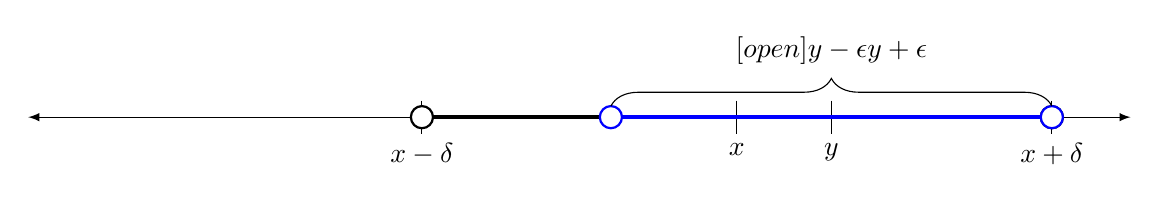
\begin{tikzpicture}[scale=2.]
          \draw[latex-latex] (-3.5,0) -- (3.5,0) ;
          \draw[shift={(1,0)},color=black] (0pt,3pt) -- (0pt,-3pt) node[below] {$x$};
          \draw[shift={(-1,0)},color=black] (0pt,3pt) -- (0pt,-3pt) node[below] {$x-\delta$};
          \draw[shift={(3,0)},color=black] (0pt,3pt) -- (0pt,-3pt) node[below] {$x+\delta$};
          \draw[very thick] (-1,0) -- (3,0);
          \path [draw=black, fill=white, thick] (-1,0) circle (2pt);
          \path [draw=black, fill=white, thick] (3,0) circle (2pt);

          \draw[shift={(1.6,0)},color=black] (0pt,3pt) -- (0pt,-3pt) node[below] {$y$};
          \draw[very thick,color=blue] (0.2,0) -- (3,0);
          \path [draw=blue, fill=white, thick] (0.2,0) circle (2pt);
          \path [draw=blue, fill=white, thick] (3,0) circle (2pt);
          
          \draw [decorate,decoration={brace,amplitude=10pt},yshift=2pt] (0.2,0) -- (3,0) node [black,midway,yshift=20pt] {$\interval[open]{y-\epsilon}{y+\epsilon}$};
        \end{tikzpicture}
      \end{figure}
      $\interval[open]{y-\epsilon}{y+\epsilon}$ is dan een deel van $\interval[open]{x-\delta}{x+\delta}$ en van $A$ bijgevolg zit $y$ in $V$.
      $V$ is dus een open deelverzameling van $A$ en daarom een deel van $\mathring{A}$.
    \item Elke open deelverzameling $W$ van $A$ is een deel van $V$: $V$ is dus het grootst.\\
      Als $W$ leeg is, is dit evident.
      Als $W$ niet leeg is, bestaat er een $x\in W$.
      Omdat $W$ open is bestaat er dan een $\delta\in \mathbb{R}_{0}^{+}$ zodat $\interval[open]{x-\delta}{x+\delta}$ een deel is van $W$ en dus van $A$.
      Dit betekent dat $x$ tot $V$ behoort.
      $W$ is een willekeurige open deelverzameling van $A$, dus ook $\mathring{A}$ is een deel van $V$.
    \end{itemize}
    We concluderen dat $\mathring{A}$ inderdaad gelijk is aan $V$.
  \end{proof}
\end{bpr}

\begin{bpr}
  Zij $A$ een deelverzameling van $\mathbb{R}$, dan ziet $\bar{A}$ er als volgt uit:
  \[ \bar{A} = \{ x\in \mathbb{R} \mid \forall \delta \in \mathbb{R}_{0}^{+}:\ \interval[open]{x-\delta}{ x+\delta} \cap A \neq \emptyset \} \]

  \begin{proof}
    Noem het rechterlid $\mathbb{R}$.
    \begin{itemize}
    \item $\mathbb{R}$ is een gesloten oververzameling van $A$.\\
      $A$ is duidelijk een deelverzameling van $\mathbb{R}$.
      We beweren dus nog dat $\mathbb{R}$ gesloten is, of dus dat $\mathbb{R}^{c}$ open is.
      Als $\mathbb{R}^{c}$ leeg is, is $\mathbb{R}$ zeker gesloten.\stref{st:r-open-en-gesloten}
      Als $\mathbb{R}^{c}$ niet leeg is, bestaat er een $\delta$ zodat $\interval[open]{x-\delta}{x+\delta} \cap A$ leeg is.
      $\interval[open]{x-\delta}{x+\delta}$ zit dus in $A^{c}$ en bijgevolg in $\mathbb{R}^{c}$.\waarom
      $\mathbb{R}$ is dus een gesloten oververzameling van $A$: $\bar{A} \subseteq \mathbb{R}$.
    \item Elke gesloten oververzameling $G$ van $A$ is een oververzameling van $\mathbb{R}$.\\
      $G^{c}$ is dan een deel van $A^{c}$.
      We beweren dat $G^{c}$ een deel is van $\mathbb{R}^{c}$.
      Als $G^{c}$ leeg is, is dit triviaal waar.
      Als $G^{c}$ niet leeg is, dan bestaat er een $x\in G^{c}$.
      Omdat $G$ gesloten is, is $G^{c}$ open en dus kunnen we een $\delta \in \mathbb{R}_{0}^{+}$ vinden zodat $\interval[open]{x-\delta}{x+\delta}$ een deel is van $G^{c}$ en dus van $A^{c}$.
      De doorsnede van $\interval[open]{x-\delta}{x+\delta}$ en $A$ is dus leeg en daarom is $x$ een element van $\mathbb{R}^{c}$.
      We vinden $G^{c}\subseteq \mathbb{R}^{c}$ en daarom $\mathbb{R} \subseteq G$.
      Omdat dit geldt voor elke gesloten oververzameling $G$, geldt het ook voor $\mathbb{R}$: $\mathbb{R} \subseteq \bar{A}$.
    \end{itemize}
    We concluderen dat $\bar{A}$ inderdaad gelijk is aan $\mathbb{R}$.
  \end{proof}
\end{bpr}

\begin{de}
  We noemen een punt $x$ van niet-lege deelverzameling $A$ van $\mathbb{R}$ een \term{inwendig punt} van $A$ als het tot $\mathring{A}$ behoort.
  \[ \exists \delta \in \mathbb{R}_{0}^{+}: \interval[open]{x-\delta}{x+\delta} \subseteq A \]
\end{de}

\begin{de}
  We noemen een punt $x$ van niet-lege deelverzameling $A$ van $\mathbb{R}$ een \term{adherent punt} aan $A$ als het tot $\bar{A}$ behoort.
  \[ \forall \delta \in \mathbb{R}_{0}^{+}:\ \interval[open]{x-\delta}{x+\delta} \cap A \neq \emptyset \]
\end{de}

\begin{vb}
  Zij $A= \interval[open left]{0}{1}$.
  \begin{itemize}
  \item $\mathring{A} = \interval[open]{0}{1}$.
  \item $\overline{A} = \interval{0}{1} \cup \{2\}$
  \end{itemize}
\end{vb}

\begin{vb}
  Zij $A= \left\{ \frac{1}{n} \mid n\in \mathbb{N}_{0} \right\}$.
  \begin{itemize}
  \item $\mathring{A} = \emptyset$.
  \item $\overline{A} = A \cup \{ 0 \}$
  \end{itemize}
\end{vb}


\begin{bpr}
  Zij $A$ een deel van $\mathbb{R}$ en $x\in \mathbb{R}$, dan behoort $x$ tot $\bar{A}$ als en slechts als er een rij $(x_{n})_{n}$ in $A$ bestaat met $x$ als limiet.

  \begin{proof}
    Bewijs van een equivalentie:
    \begin{itemize}
    \item $\Rightarrow$\\
      Zij $x$ een adherent punt.
      Als $x$ tot $A$ behoort heeft de constante rij $(x)_{n}$ $x$ als limiet.
      Stel daarom dat $x$ tot $\bar{A}\setminus A$ behoort.
      Voor elke $n\in \mathbb{N}$ is $\interval[open]{x-\frac{1}{n}}{x+\frac{1}{n}} \cap A$ niet leeg (omdat $x$ een adherent punt is).
      Kies dus voor elke $n$ een $x_{n} \in \interval[open]{x-\frac{1}{n}}{x+\frac{1}{n}}$ om een rij $(x_{n})_{n}$ te bekomen met $x$ als limiet.
    \item $\Leftarrow$\\
      Zij $(x_{n})_{n}$ een rij met limiet $x\in A$. We bewijzen dat $x$ een adherent punt is aan $A$.
      Kies daartoe een willekeurige $\delta \in \mathbb{R}_{0}^{+}$.
      Er bestaat dan een $n_{0}\in \mathbb{N}$ zodat voor alle volgende $n\in\mathbb{N}$ $x_{n}$ in $\interval[open]{x-\delta}{x+\delta}$ zit.
      Omdat $(x_{n})_{n}$ een rij is in $A$ behoort $x_{n}$ ook tot $A$.
      De doorsnede van $A$ en $\interval[open]{x-\delta}{x+\delta}$ bevat dus al zeker $x_{n}$ en is bijgevolg niet leeg.
    \end{itemize}
  \end{proof}
\end{bpr}

\begin{pr}
  \[ \mathring{\mathbb{Q}} = \emptyset \quad\text{ en }\quad \overline{\mathbb{Q}} = \mathbb{R} \]

  \begin{proof}
    Elk deel appart.
    \begin{itemize}
    \item Kies een willekeurige $q\in \mathbb{Q}$ en een willekeurige $\delta \in \mathbb{R}_{0}^{+}$, dan bevat $\interval[open]{q-\delta}{q+\delta}$ zeker irrationale getallen.\waarom
      Er bestaat dus geen enkel inwendig punt van $\mathbb{Q}$.
    \item Kies een willekeurig punt $r \in \mathbb{R}$, dan bestaat er in elke omgeving van $r$ een rationaal punt\prref{pr:q-dicht-in-r}, dus elk punt $r\in \mathbb{R}$ is adherent aan $\mathbb{R}$.
    \end{itemize}
  \end{proof}
\end{pr}


\begin{st}
  Zij $A$ een deelverzameling van $\mathbb{R}$.
  \[ \left(\mathring{A}\right)^{c} = \overline{A^{c}} \]
  
  \begin{proof}
    \[
    \begin{array}{rll}
      \left(\mathring{A}\right)^{c}
      &= \{ x\in A\mid \exists \delta \in \mathbb{R}_{0}^{+}:\ \interval[open]{x-\delta}{x+\delta} \subseteq A \}^{c}\\
      &= \{ x\in \mathbb{R}\mid (x\in A) \wedge (\exists \delta \in \mathbb{R}_{0}^{+}:\ \interval[open]{x-\delta}{x+\delta} \subseteq A) \}^{c}\\
      &= \{ x\in \mathbb{R}\mid \neg((x\in A) \wedge (\exists \delta \in \mathbb{R}_{0}^{+}:\ \interval[open]{x-\delta}{x+\delta} \subseteq A)) \}\\
      &= \{ x\in \mathbb{R}\mid \neg(x\in A) \vee \neg(\exists \delta \in \mathbb{R}_{0}^{+}:\ \interval[open]{x-\delta}{x+\delta} \subseteq A)) \}\\
      &= A^{c} \cup \{ x\in \mathbb{R} \mid \neg(\exists \delta \in \mathbb{R}_{0}^{+}:\ \interval[open]{x-\delta}{x+\delta} \subseteq A)) \}\\
      &= A^{c} \cup \{ x\in \mathbb{R} \mid \forall \delta \in \mathbb{R}_{0}^{+}:\ \interval[open]{x-\delta}{x+\delta} \cap A^{c} \neq \emptyset \} \\
      &= \{ x\in \mathbb{R} \mid \forall \delta \in \mathbb{R}_{0}^{+}:\ \interval[open]{x-\delta}{ x+\delta} \cap A^{c} \neq \emptyset \}
      &= \overline{A^{c}}\\
    \end{array}
    \]
  \end{proof}
\feed
\end{st}
\extra{geldt dit in $\mathbb{C}$?}

\begin{st}
  Zij $A$ een deelverzameling van $\mathbb{R}$.
  \[ \left(\overline{A}\right)^{c} = \mathring{\left(A^{c}\right)} \]

  \begin{proof}
    \[
    \begin{array}{rll}
      \left(\overline{A}\right)^{c}
      &= \{ x\in \mathbb{R} \mid \forall \delta \in \mathbb{R}_{0}^{+}:\ \interval[open]{x-\delta}{ x+\delta} \cap A \neq \emptyset \}^{c}\\
      &= \left\{ x\in \mathbb{R} \mid \neg\left(\forall \delta \in \mathbb{R}_{0}^{+}:\ \interval[open]{x-\delta}{ x+\delta} \cap A \neq \emptyset \right) \right\}\\
      &= \{ x\in \mathbb{R} \mid \exists \delta \in \mathbb{R}_{0}^{+}:\ \interval[open]{x-\delta}{ x+\delta} \cap A = \emptyset \}\\
      &= \{ x\in \mathbb{R} \mid \exists \delta \in \mathbb{R}_{0}^{+}:\ \interval[open]{x-\delta}{ x+\delta} \subseteq A^{c} \}
      &= \mathring{\left(A^{c}\right)}\\
    \end{array}
    \]
  \end{proof}
\feed
\extra{geldt dit in $\mathbb{C}$?}
\end{st}

\begin{st}
  Zij $A$ en $B$ deelverzamelingen van $\mathbb{R}$.
  \[ \overline{A \cap B} = \overline{A} \cap \overline{B} \]

  \begin{proof}
    \[
    \begin{array}{rll}
      \overline{A \cap B} 
      &= \{ x\in \mathbb{R} \mid \forall \delta \in \mathbb{R}_{0}^{+}:\ \interval[open]{x-\delta}{ x+\delta} \cap (A \cap B) \neq \emptyset \}\\
      &= \{ x\in \mathbb{R} \mid \forall \delta \in \mathbb{R}_{0}^{+}:\ ((\interval[open]{x-\delta}{ x+\delta} \cap A) \cap (\interval[open]{x-\delta}{ x+\delta} \cap B)) \neq \emptyset \}\\
      &= \{ x\in \mathbb{R} \mid \forall \delta \in \mathbb{R}_{0}^{+}:\ ((\interval[open]{x-\delta}{ x+\delta} \cap A) \neq 0 \wedge (\interval[open]{x-\delta}{ x+\delta} \cap B) \neq \emptyset \}
      &= \overline{A} \cap \overline{B} \\
    \end{array}
    \]
  \end{proof}
\feed
\extra{geldt dit in $\mathbb{C}$?}
\end{st}

\begin{st}
  Zij $A$ en $B$ deelverzamelingen van $\mathbb{R}$.
  \[ \overline{A \cup B} = \overline{A} \cup \overline{B} \]

  \begin{proof}
    \[
    \begin{array}{rll}
      \overline{A \cap B} 
      &= \{ x\in \mathbb{R} \mid \forall \delta \in \mathbb{R}_{0}^{+}:\ \interval[open]{x-\delta}{ x+\delta} \cap (A \cup B) \neq \emptyset \}\\
      &= \{ x\in \mathbb{R} \mid \forall \delta \in \mathbb{R}_{0}^{+}:\ ((\interval[open]{x-\delta}{ x+\delta} \cap A) \cup (\interval[open]{x-\delta}{ x+\delta} \cap B)) \neq \emptyset \}\\
      &= \{ x\in \mathbb{R} \mid \forall \delta \in \mathbb{R}_{0}^{+}:\ ((\interval[open]{x-\delta}{ x+\delta} \cap A) \neq 0 \vee (\interval[open]{x-\delta}{ x+\delta} \cap B) \neq \emptyset \}
      &= \overline{A} \cup \overline{B} \\
    \end{array}
    \]
  \end{proof}
\feed
\extra{geldt dit in $\mathbb{C}$?}
\end{st}


\begin{st}
  Zij $A$ en $B$ deelverzamelingen van $\mathbb{R}$.
  \[ \mathring{\left(A \cap B\right)} = \mathring{A} \cap \mathring{B} \]

\extra{bewijs}
\extra{geldt dit in $\mathbb{C}$?}
\end{st}

\begin{st}
  Zij $A$ en $B$ deelverzamelingen van $\mathbb{R}$.
  \[ \mathring{\left(A \cup B\right)} = \mathring{A} \cup \mathring{B} \]

\extra{bewijs}
\extra{geldt dit in $\mathbb{C}$?}
\end{st}


\subsection{Randpunten, ge\"isoleerde punten en ophopingspunten.}
\label{sec:randp-geis-punt}

\begin{de}
  De \term{rand} $\partial A$ van een deelverzameling $A$ van $\mathbb{R}$ definieren we als volgt:
  \[ \partial A = \bar{A} \setminus \mathring{A} \]
\end{de}

\begin{de}
  Een \term{randpunt} van een deelverzameling $A$ van $\mathbb{R}$ is een element van de rand $\partial A$ van $A$.
\end{de}

\begin{opm}
  Een randpunt van $A$ hoeft niet tot $A$ te behoren.
\extra{voorbeeld}
\end{opm}

\begin{st}
  Een punt $x\in \mathbb{R}$ is een randpunt van een deelverzameling $A$ van $\mathbb{R}$ als en slechts het volgende geldt:
  \[ \forall \delta \in \mathbb{R}_{0}^{+}:\ \interval[open]{x-\delta}{x+\delta} \cap A \neq \emptyset\ \wedge\  \interval[open]{x-\delta}{x+\delta} \cap A^{c} \neq \emptyset \]

  \begin{proof}
    Een randpunt $x$ van een deelverzameling $A$ van $\mathbb{R}$ is een adherent punt dat geen inwendig punt is.
    Het eerste deel van de conjunctie is waar omdat $A$ een adherent punt is.
    Omdat $A$ geen inwendig punt is geldt het volgende:
    \[ \forall \delta \in \mathbb{R}_{0}^{+}: \interval[open]{x-\delta}{x+\delta} \not\subseteq A \]
    Dit betekent dat er voor elke $\delta \in \mathbb{R}_{0}^{+}$ een element in $\interval[open]{x-\delta}{x+\delta}$ niet tot $A$ behoort (maar dus wel tot $A^{c}$).
    De doorsnede van $\interval[open]{x-\delta}{x+\delta}$ en $A^{c}$ is dus niet leeg.
  \end{proof}
\end{st}

\begin{de}
  Zij $A$ een niet-lege deelverzameling van $\mathbb{R}$, dan noemen we een punt $x\in A$ een \term{ge\"isoleerd punt} van $A$ als het volgende geldt:
  \[ \exists \delta \in \mathbb{R}_{0}^{+}:\ \interval[open]{x-\delta}{x+\delta} \cap A = \{ x \} \]
\end{de}

\begin{de}
  Zij $A$ een niet-lege deelverzameling van $\mathbb{R}$, dan noemen we een punt $x\in A$ een \term{ophopingspunt} of \term{accumulatiepunt} van $A$ als het volgende geldt:
  \[ \forall \delta \in \mathbb{R}_{0}^{+}:\ \interval[open]{x-\delta}{x+\delta} \cap (A \setminus \{x\}) \neq \emptyset \]
\end{de}

\begin{opm}
  Eer ophopingspunt van $A$ hoeft niet tot $A$ te behoren.
\extra{voorbeeld}
\end{opm}

\begin{opm}
  Een punt $x$ in een niet-lege deelverzameling $A$ van $\mathbb{R}$, dan is $x$ ofwel een ge\"isoleerd punt, ofwel een ophopingspunt.
  De definities zijn immers de negatie van elkaar.
\end{opm}

\begin{vb}
  Zij $A= \interval[open left]{0}{1} \cup \{2\}$.
  \begin{itemize}
  \item $\partial{A} = \{0\} \cup \{1\} \cup \{2\}$
  \item De ge\"isoleerde punten van $A$ zijn $\{2\}$.
  \item De ophopingspunten van $A$ zijn $\interval{0}{1}$.
  \end{itemize}
\end{vb}

\begin{vb}
  Zij $A= \left\{ \frac{1}{n} \mid n\in \mathbb{N}_{0} \right\}$.
  \begin{itemize}
  \item $\partial{A} = \overline{A}$
  \item Alle punten van $A$ zijn ge\"isoleerde punten.
  \item De ophopingspunten van $A$ zijn $\interval{0}{1}$.
  \end{itemize}
\end{vb}

\begin{bpr}
  \label{pr:equivalenties-ophopingspunt}
  Zij $A$ een niet een niet-lege deelverzameling van $\mathbb{R}$, dan zijn volgende uitspraken equivalent.
  \begin{enumerate}
  \item $x$ is een ophopingspunt van $A$.
  \item Voor alle $\delta > 0$ bevat $\interval[open]{x-\delta}{x+\delta} \cap A$ oneindig veel punten.
  \item Er bestaat een rij $(x_{n})_{n}$ in $A\setminus \{x\}$ die naar $x$ convergeert.  
  \end{enumerate}

  \begin{proof}
    Equivalentie vanuit circulaire implicaties
    \begin{itemize}
    \item $(1) \Rightarrow (3)$\\
      Uit de definite van een ophopingspunt volgt dat voor elke $n\in \mathbb{N}$ de verzameling $\interval[open]{x-\frac{1}{n}}{x+\frac{1}{n}}\cap (A \setminus \{x\})$ niet leeg is.
      Voor elke $n$ kunnen we er dus een $x_{n}$ in kiezen om een rij $(x_{n})_{n}$ te construeren die $x$ als limiet heeft.
    \item $(3) \Rightarrow (2)$\\
      Stel dat er een $\delta \in \mathbb{R}_{0}^{+}$ bestaat zodat $\interval[open]{x-\delta}{x+\delta} \cap A$ eindig is, dan bestaat er in die verzameling een punt dat het dichtst bij $x$ ligt.
      Noem dit punt $y$ en noem de afstand tot $x$ $\epsilon = |y-x|$.
      Dit houdt in dat de verzameling $\interval[open]{x-\epsilon}{x+\epsilon} \cap A$ leeg is.
      Omdat de rij $(x_{n})_{n}$ in $A\setminus \{x\}$ naar $x$ convergeert, moet er echter een $n_{0}\in\mathbb{N}$ bestaan zodat alle voor volgende $n\in \mathbb{N}$ $x_{n}$ in $\interval[open]{x-\epsilon}{x+\epsilon}$ moet liggen.
      Omdat de rij in  $A\setminus \{x\}$ ligt moeten die $x_{n}$ dus ook in $\interval[open]{x-\epsilon}{x+\epsilon} \cap A$ liggen, maar dit is in tegenspraak met het feit dat deze verzameling leeg is.
    \item $(2) \Rightarrow (1)$\\
      Voor elke $\delta \in \mathbb{R}_{0}^{+}$ bevat $\interval[open]{x-\delta}{x+\delta} \cap A$ oneindig veel punten.
      $\interval[open]{x-\delta}{x+\delta} \cap (A \setminus \{x\})$ bevat dan nog steeds oneindig veel punten en is dus niet leeg.
    \end{itemize}
  \end{proof}
\end{bpr}

\begin{bst}
  De \term{stelling van Bolzano-Weierstra\ss} (ophopingspuntversie).
  Elk oneindig begrensd deel van $\mathbb{R}$ heeft minstens \'e\'en ophopingspunt.

  \begin{proof}
    Zij $A$ een oneindige begrensde deelverzameling van $\mathbb{R}$.
    Kies nu een aftelbaar oneindige deelverzameling $B$ van $A$ en nummer de elementen van $B$ om een rij $(x_{n})_{n}$ te bekomen.
    Merk op dat die rij in $A$ ligt en dus begrensd is.
    Er bestaat dus een convergente deelrij $(x_{n_{k}})_{k}$\stref{st:bolzano-rijen}.
    Noem de limiet van deze deelrij $x$.
    We beweren dat $x$ een ophopingspunt is van $A$.
    Kies nu een $\delta \in \mathbb{R}_{0}^{+}$.
    Er bestaat dan een $k_{0}\in\mathbb{N}$ zodat voor alle volgende $k\in \mathbb{N}$ $x_{n_{k}}$ dichter dan $\delta$ bij $x$ ligt.
    Het interval $\interval[open]{x-\delta}{x+\delta}$ bevat dan oneindig veel punten (tenminste alle $x_{n_{k}}$ met $k>k_{0}$).
    Bijgevolg is $x$ een ophopingspunt van $A$.\prref{pr:equivalenties-ophopingspunt}
  \end{proof}
\end{bst}

\begin{st}
  Elke overaftelbare deelverzameling van $\mathbb{R}$ heeft minstens \'e\'en ophopingspunt.

  \begin{proof}
    Contrapositie: Elke deelverzameling van $\mathbb{R}$ zonder ophopingspunten is aftelbaar.\\
    Zij $V$ een deelverzameling van $\mathbb{R}$ zonder ophopingspunten.
    Als $V$ leeg is is $V$ zeker aftelbaar.
    Als $V$ eindig is, is $V$ ook zeker aftelbaar.
    Stel daarom dat $V$ oneindig is.
    Omdat $V$ geen ophopingspunten bevat kunnen we een willekeurig punt $x$ kiezen van $V$ opdat dat punt geen ophopingspunt is: ($x$ is dan een ge\"isoleerd punt.)
    \[ \exists \delta \in \mathbb{R}_{0}^{+}:\ \interval[open]{x-\delta}{x+\delta} \cap A = \{x\} \]
    Noem $x$ punt $1$: $p_{0} = x$.
    Noem $p_{1} = \max( V \cap \interval[open left]{-\infty}{p_{0}})$ als het bestaat. Sta deze stap over als dat maximum niet bestaat.
    Noem $p_{2} = \min(V \cap \interval[open right]{p_{1}}{+\infty})$ als het bestaat.
    Sta deze stap over als dat minimum niet bestaat.
    Merk op dat minstens \'e\'en van de punten $p_{1}$ en $p_{2}$ moet bestaan.
    We beweren nu dat we, door afwisselend links en rechts punten te kiezen van de huidige $p_{i}$, alle punten van $V$ kunnen opsommen.
    Stel immers dat we $V$ niet zouden kunnen opsommen op deze manier.
    T.t.z dat er een punt $y\in V$ bestaat dat niet tussen de $p_{i}$ zit.
    Dat punt is ofwel groter, ofwel kleiner dan $x$.
    Stel dat $y$ kleiner is dan $x$, de andere redenering gaat analoog.
    Omdat $V$ geen ophopingspunten bevat, bestaat er dan een punt $y_{1}\in V$ dat het dichtst bij $y=y_{0}$ ligt aan de rechterkant.
    Da punt $y_{1}$ kan ook niet in de lijst $p_{i}$ zitten, want anders zou $y$ per constructie in de lijst hebben gezeten.
    We kunnen opnieuw een punt $y_{2}$, rechts van $y_{1}$ kiezen en zo verder gaan om een oneindige lijst $y_{i}$ op te bouwen van punten, kleiner dan $x$ en niet in de lijst $p_{i}$.
    Omdat de rij $(y_{i})_{i}$ stijgend en begrensd is, moet hij convergeren, maar de limiet zou dan een ophopingspunt van $V$ zijn en dat is in tegenspraak met de keuze van $V$.
  \end{proof}
\feed
\end{st}

\begin{figure}[H]
  \centering
  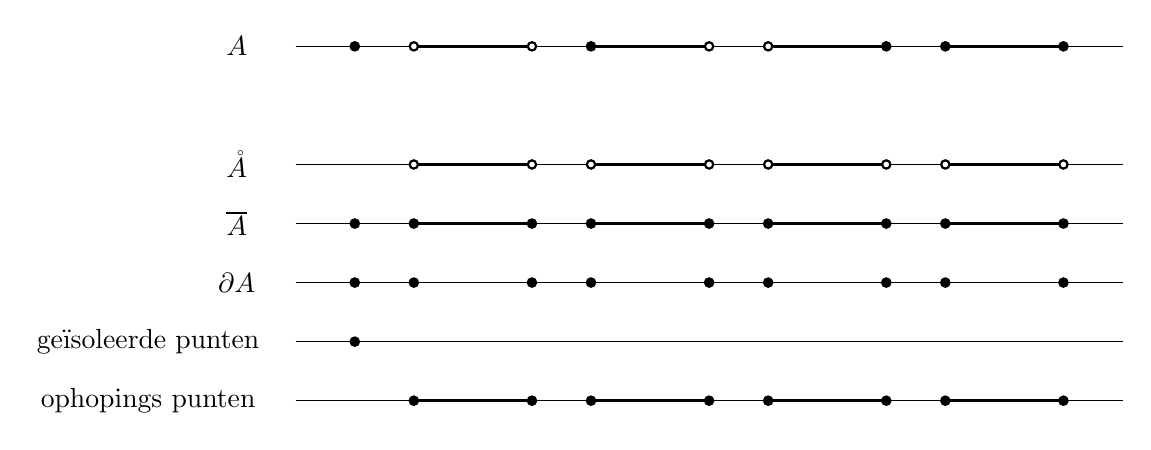
\begin{tikzpicture}[scale=.75]
    \draw (-6,0) node {$A$};
    \draw (-5,0) -- (9,0) ;

    \path [draw=black, fill=black, thick] (-4,0) circle (2pt);

    \draw[very thick] (-3,0) -- (-1,0);
    \path [draw=black, fill=white, thick] (-3,0) circle (2pt);
    \path [draw=black, fill=white, thick] (-1,0) circle (2pt);

    \draw[very thick] (0,0) -- (2,0);
    \path [draw=black, fill=black, thick] (0,0) circle (2pt);
    \path [draw=black, fill=white, thick] (2,0) circle (2pt);

    \draw[very thick] (3,0) -- (5,0);
    \path [draw=black, fill=white, thick] (3,0) circle (2pt);
    \path [draw=black, fill=black, thick] (5,0) circle (2pt);

    \draw[very thick] (6,0) -- (8,0);
    \path [draw=black, fill=black, thick] (6,0) circle (2pt);
    \path [draw=black, fill=black, thick] (8,0) circle (2pt);


    \draw (-6,-2) node {$\mathring{A}$};
    \draw (-5,-2) -- (9,-2) ;

    \draw[very thick] (-3,-2) -- (-1,-2);
    \path [draw=black, fill=white, thick] (-3,-2) circle (2pt);
    \path [draw=black, fill=white, thick] (-1,-2) circle (2pt);

    \draw[very thick] (0,-2) -- (2,-2);
    \path [draw=black, fill=white, thick] (0,-2) circle (2pt);
    \path [draw=black, fill=white, thick] (2,-2) circle (2pt);

    \draw[very thick] (3,-2) -- (5,-2);
    \path [draw=black, fill=white, thick] (3,-2) circle (2pt);
    \path [draw=black, fill=white, thick] (5,-2) circle (2pt);

    \draw[very thick] (6,-2) -- (8,-2);
    \path [draw=black, fill=white, thick] (6,-2) circle (2pt);
    \path [draw=black, fill=white, thick] (8,-2) circle (2pt);


    \draw (-6,-3) node {$\overline{A}$};
    \draw (-5,-3) -- (9,-3) ;

    \path [draw=black, fill=black, thick] (-4,-3) circle (2pt);

    \draw[very thick] (-3,-3) -- (-1,-3);
    \path [draw=black, fill=black, thick] (-3,-3) circle (2pt);
    \path [draw=black, fill=black, thick] (-1,-3) circle (2pt);

    \draw[very thick] (0,-3) -- (2,-3);
    \path [draw=black, fill=black, thick] (0,-3) circle (2pt);
    \path [draw=black, fill=black, thick] (2,-3) circle (2pt);

    \draw[very thick] (3,-3) -- (5,-3);
    \path [draw=black, fill=black, thick] (3,-3) circle (2pt);
    \path [draw=black, fill=black, thick] (5,-3) circle (2pt);

    \draw[very thick] (6,-3) -- (8,-3);
    \path [draw=black, fill=black, thick] (6,-3) circle (2pt);
    \path [draw=black, fill=black, thick] (8,-3) circle (2pt);


    \draw (-6,-4) node {$\partial{A}$};
    \draw (-5,-4) -- (9,-4) ;

    \path [draw=black, fill=black, thick] (-4,-4) circle (2pt);

    \path [draw=black, fill=black, thick] (-3,-4) circle (2pt);
    \path [draw=black, fill=black, thick] (-1,-4) circle (2pt);

    \path [draw=black, fill=black, thick] (0,-4) circle (2pt);
    \path [draw=black, fill=black, thick] (2,-4) circle (2pt);

    \path [draw=black, fill=black, thick] (3,-4) circle (2pt);
    \path [draw=black, fill=black, thick] (5,-4) circle (2pt);

    \path [draw=black, fill=black, thick] (6,-4) circle (2pt);
    \path [draw=black, fill=black, thick] (8,-4) circle (2pt);


    \draw (-7.5,-5) node {ge\"isoleerde punten};
    \draw (-5,-5) -- (9,-5) ;

    \path [draw=black, fill=black, thick] (-4,-5) circle (2pt);

    \draw (-7.5,-6) node {ophopings punten};
    \draw (-5,-6) -- (9,-6) ;

    \draw[very thick] (-3,-6) -- (-1,-6);
    \path [draw=black, fill=black, thick] (-3,-6) circle (2pt);
    \path [draw=black, fill=black, thick] (-1,-6) circle (2pt);

    \draw[very thick] (0,-6) -- (2,-6);
    \path [draw=black, fill=black, thick] (0,-6) circle (2pt);
    \path [draw=black, fill=black, thick] (2,-6) circle (2pt);

    \draw[very thick] (3,-6) -- (5,-6);
    \path [draw=black, fill=black, thick] (3,-6) circle (2pt);
    \path [draw=black, fill=black, thick] (5,-6) circle (2pt);

    \draw[very thick] (6,-6) -- (8,-6);
    \path [draw=black, fill=black, thick] (6,-6) circle (2pt);
    \path [draw=black, fill=black, thick] (8,-6) circle (2pt);


  \end{tikzpicture}
\caption{Illustratie van sluiting, inwendige, randpunten, ophopingspunten en ge\"isoleerde punten}
\end{figure}


\subsection{Relatieve topologie}
\label{sec:relatieve-topologie}

\begin{de}
  We noemen een deelverzameling $A$ van $X\subseteq \mathbb{R}$ \term{relatief open} in $X$ als het volgende geldt:
  \[ \forall x\in A:\ \exists \delta \in \mathbb{R}_{0}^{+}:\ \forall y\in X:\ |y-x| < \delta \Rightarrow y \in A \]
\end{de}

\begin{st}
  Een  deelverzameling $A$ van $X\subseteq \mathbb{R}$  is relatief open in $X$ als en slechts als het volgende geldt:
  \[ \forall x\in A:\ \exists \delta\in \mathbb{R}_{0}^{+}:\ \interval[open]{x-\delta}{x+\delta} \cap X \subseteq A \]
  \extra{bewijs}
\end{st}

\begin{vb}
  Beschouw $\interval[open right]{0}{1}$ als deelverzameling van $\interval[open right]{0}{2}$.
  \begin{itemize}
  \item $\interval[open right]{0}{1}$ is relatief open in $\interval[open right]{0}{2}$.
    $\interval[open right]{0}{1}$ is niet open in $\mathbb{R}$ omdat er geen punten links van $0$ in liggen, maar in $\interval[open right]{0}{2}$ liggen ook geen punten links van $0$, dus dat is geen probleem.
  \item $\interval[open right]{1}{2}$ is dan relatief gesloten.
  \end{itemize}
\end{vb}

\begin{de}
  We noemen een deelverzameling $A$ van $X\subseteq \mathbb{R}$ \term{relatief gesloten} in $X$ als het relatief complement $X\setminus B$ van $B$ relatief open is in $X$.
\end{de}

\begin{pr}
  Zij $X$ een niet-leeg deel van $\mathbb{R}$ en $A \subseteq X$.
  $A$ is relatief open in $X$ als en slechts als er een open $V\subseteq \mathbb{R}$ bestaat zodat $A=V \cap X$ geldt.

  \begin{proof}
    Bewijs van een equivalentie\\
    \begin{itemize}
    \item $\Rightarrow$\\
      Als $A$ leeg is kunnen we voor $V$ $\emptyset$ nemen.
      Als $A$ niet leeg is, dan bestaat er een $x\in A$.
      We kunnen dan een $\delta_{x}$ kiezen zodat $\interval[open]{x-\delta}{x+\delta} \cap X$ een deel is van $A$.
      Benoem nu $V$ als volgt:
      \[ \bigcup_{x\in A}\interval[open]{x-\delta_{x}}{x+\delta_{x}} \]
      $V$ is dan een open deel van $\mathbb{R}$ want het is een unie van open verzamelingen.\prref{pr:unie-open-verzamelingen-open}
      Bovendien is $A$ per constructie de doorsnede van $V$ en $X$.
    \item $\Leftarrow$\\
      Zij $X$ een niet-leeg deel van $\mathbb{R}$ en $V$ een open deel van $\mathbb{R}$.
      We bewijzen dan dat $A$ relatief open is in $V\cap X$.
      Kies daartoe een $x\in A$. Er bestaat dan een $\delta\in \mathbb{R}_{0}^{+}$ zodat $\interval[open]{x-\delta}{x+\delta}$ in $V$ zit.
      De doorsnede van dit interval en $X$ is dan een deel van $V \cap X$.
      $V\cap X$ is dus een open deel van $X$.
    \end{itemize}
  \end{proof}
\end{pr}

\begin{pr}
  Zij $X$ een niet-leeg deel van $\mathbb{R}$ en $A \subseteq X$.
  $A$ is relatief gesloten in $X$ als en slechs als er een gesloten $\mathbb{R} \subseteq \mathbb{R}$ bestaat zodat $A=\mathbb{R} \cap X$ geldt.
  \TODO{oefening}
\end{pr}

\extra{mogelijke stelling: unie van relatief open verzamelingen is open}
\extra{mogelijke stelling: eindige doorsnede van relatief open verzamelingen is open}
\extra{mogelijke stelling: doorsnede van relatief gesloten verzamelingen is gesloten}
\extra{mogelijke stelling: eindige unie van relatief gesloten verzamelingen is gesloten}
\extra{mogelijke stelling: relatief gesloten asa limiet van elke convergente rij erin}
\extra{mogelijke stelling: relatief gesloten en begrensd als elke rij erin een convergente deelrij heeft met limiet erin}


\section{Complexe getallen}
\label{sec:de-complexe-getallen}

\subsection{Rijen in $\mathbb{C}$}
\label{sec:rijen-mathbbc}

\begin{de}
  We zeggen dat een rij $(x_{n})_{n}$ in $\mathbb{C}$ \term{convergeert} naar een element $c\in \mathbb{C}$ als en slechts als het volgende geldt:
  \[ \forall \epsilon \in \mathbb{R}_{0}^{+}:\ \exists n_{0}\in \mathbb{N}:\ \forall n\in \mathbb{N}:\ n \ge n_{0} \Rightarrow |z_{n}-c| < \epsilon \]
  We noemen $c$ de \term{limiet} van de rij $(x_{n})_{n}$.
  \[ \lim_{n\rightarrow +\infty}z_{n} = c \]
\end{de}

\begin{de}
  Een rij die convergeert noemen we een \term{convergente} rij.
\end{de}

\begin{pr}
  \label{pr:complexe-limiet-splitsen}
  Zij $(z_{n})_{n}$ een rij in $\mathbb{C}$.
  Noem $x_{n} = Re(z_{n})$ en $y_{n} = Im(z_{n})$.
  Noem bovendien $a=Re(c)$ en $b=Im(c)$.
  $(z_{n})_{n}$ convergeert naar $c$ als en slechts als $(x_{n})_{n}$ naar $a$ en $(y_{n})_{n}$ naar $b$ convergeert.

  \begin{proof}
    Merk eerst op dat de volgende ongelijkheid geldt door $x_{n}$, $a$, $y_{n}$ en $b$ te beschouwen als complexe getallen.\prref{pr:tweede-driehoeksongelijkheid-C}
    \[ |z_{n}-c| \le |x_{n}-a| + |y_{n}-b| \]
    Er gelden ook de volgende ongelijkheden.\prref{pr:reel-deel-kleine}\prref{pr:imaginair-deel-kleiner}
    \[ |x_{n}-a| \le |z_{n}-c| \]
    \[ |y_{n}-b| \le |z_{n}-c| \]
    \begin{itemize}
    \item $\Rightarrow$
      Kies een wilekeurige $\delta \in \mathbb{R}_{0}^{+}$.
      Vanwege de tweede en derde ongelijkheid worden $|x_{n}-a|$ en $|y_{n}-b|$ kleiner dan $\delta$ vanaf een bepaalde $n\in \mathbb{N}$ omdat $z_{n}$ convergeert naar $c$.
    \item $\Leftarrow$
      Kies een willekeurige $\delta \in \mathbb{R}_{0}^{+}$.
      Er bestaan dan een $n_{x},n_{y}\in \mathbb{N}$ zodat $|x_{n}-a|$ en $|y_{n}-b|$ kleiner worden dan $\frac{\delta}{2}$ voor $n$ groter dan $n_{x}$, respectievelijk $n_{y}$.
      Vanaf $\max\{n_{x},n_{y}\}$ geldt dan het volgende vanwege de eerste ongelijkheid:
      \[ |z_{n}-c| \le |x_{n}-a| + |y_{n}-b| < \frac{\delta}{2}+\frac{\delta}{2} = \delta \]
    \end{itemize}
  \end{proof}
  \extra{dit kan mooier?}
\end{pr}

\begin{st}
  \label{st:bolzano-complexe-rijen}
  De \term{stelling van Bolzano-Weierstra\ss} voor complexe rijen\\
  Elke begrensde rij in $\mathbb{C}$ heeft een convergente deelrij.

  \begin{proof}
    Zij $(z_{n})_{n}$ een begrensde rij in $\mathbb{C}$
    Noem $x_{n} = Re(z_{n})$ en $y_{n} = Im(z_{n})$.
    De rijen $(x_{n})_{n}$ en $(y_{n})_{n}$ zijn dan begrensde rijen in $\mathbb{R}$\prref{pr:tweede-driehoeksongelijkheid-C}
    We kunnen van $(x_{n})_{n}$ een convergente deelrij $(x_{n_{k}})_{k}$ met limiet $a$ nemen\stref{st:bolzano-rijen}.
    We kunnen dan van $(y_{n_{k}})_{k}$ een convergente deelrij $(y_{n_{k_{l}}})_{l}$ nemen met limiet $b$
    Noem de limieten respectievelijk $a$ en $b$.
    De deelrij $(z_{n_{k_{l}}})_{l}$ van $(z_{n})_{n}$ convergeert dan naar $a+bi$.\prref{pr:complexe-limiet-splitsen}
  \end{proof}
\end{st}

\begin{de}
  We noemen een rij $(z_{n})_{n}$ in $\mathbb{C}$ een \term{Cauchyrij} als en slechts als het volgende geldt:
  \[ \forall \epsilon \in \mathbb{R}_{0}^{+}:\ \exists n_{0}\in \mathbb{N}:\ \forall n,m\in \mathbb{N}_{0}: n,m\ge n_{0} \Rightarrow |z_{n}-z_{m}| < \epsilon \]
\end{de}

\begin{pr}
  Zij $(z_{n})_{n}$ een rij in $\mathbb{C}$.
  Noem $x_{n} = Re(z_{n})$ en $y_{n} = Im(z_{n})$.
  $(z_{n})_{n}$ is een Cauchyrij als en slechts als $(x_{n})_{n}$ en $(y_{n})_{n}$ Cauchyrijen zijn.

  \begin{proof}
    We beginnen opnieuw met drie ongelijkheden:
    \[ |z_{n}-z_{m}| \le |x_{n}-x_{m}| + |y_{n}-y_{m}| \]
    \[ |x_{n}-x_{m}| \le |z_{n}-z_{m}| \]
    \[ |y_{n}-y_{m}| \le |z_{n}-z_{m}| \]
    \begin{itemize}
    \item $\Rightarrow$\\
      Kies een willekeurige $\delta \in \mathbb{R}_{0}^{+}$.
      Vanwege de tweede en derde ongelijkheid worden $|x_{n}-x_{m}|$ en $|y_{n}-y_{m}|$ kleiner dan $\delta$ vanaf een bepaalde $n\in \mathbb{N}$ omdat $z_{n}$ een Cauchyrij is.
    \item $\Leftarrow$\\
      Kies een willekeurige $\delta \in \mathbb{R}_{0}^{+}$.
      Er bestaan dan een $n_{x},n_{y}\in \mathbb{N}$ zodat $|x_{n}-x_{m}|$ en $|y_{n}-y_{m}|$ kleiner worden dan $\frac{\delta}{2}$ voor $n,m$ groter dan $n_{x}$, respectievelijk $n_{y}$.
      Vanaf $\max\{n_{x},n_{y}\}$ geldt dan het volgende vanwege de eerste ongelijkheid:
      \[ |z_{n}-z_{m}| \le |x_{n}-x_{m}| + |y_{n}-y_{m}| < \frac{\delta}{2}+\frac{\delta}{2} = \delta \]
    \end{itemize}
  \end{proof}
\end{pr}

\begin{st}
  Een rij $(z_{n})_{n}$ in $\mathbb{C}$ is convergent als en slechts als het een Cauchyrij is.

  \begin{proof}
    Bewijs van een equivalentie\\
    \begin{itemize}
    \item $\Rightarrow$\\
\extra{bewijs}
    \item $\Leftarrow$\\
      Noem $x_{n} = Re(z_{n})$ en $y_{n} = Im(z_{n})$.
      $(x_{n})_{n}$ en $(y_{n})_{n}$ zijn dan Cauchyrijen in $\mathbb{R}$, en convergeren dus.\prref{pr:cauchyrij-in-R-convergeert}
      Noem $a$ en $b$ de respectievelijke limieten.
      $(z_{n})_{n}$ convergeert dan naar $a+bi$.\prref{pr:complexe-limiet-splitsen}
    \end{itemize}
  \end{proof}
\end{st}


\subsection{Topologie in $\mathbb{C}$}
\label{sec:topologie-mathbbc}

\begin{de}
  We noemen een deelverzameling $A$ van $\mathbb{C}$ \term{open} als en slechts als het volgende geldt:
  \[ \forall x\in A:\ \exists \delta \in \mathbb{R}_{0}^{+}:\ \forall y\in \mathbb{C}:\ |y-x| < \delta \Rightarrow y \in A \]
\end{de}

\begin{de}
  We noemen een deelverzameling $A$ van $\mathbb{C}$ \term{gesloten} als en slechts als $\mathbb{C} \setminus A$ open is in $\mathbb{C}$.
\end{de}

\begin{de}
  Een (open) \term{cirkelschijf} in $\mathbb{C}$ met middelpunt $m\in \mathbb{C}$ en straal $r\in \mathbb{R}_{0}^{+}$ is de verzameling $C$:
  \[ C = \{ z \in \mathbb{C} \mid |z-m| < r \} \]
\end{de}

\begin{st}
  Een open cirkelschijf in $\mathbb{C}$ is een open deelverzameling van $\mathbb{C}$.

  \begin{proof}
    Kies een willekeurige $x$ in een cirkelschijf $A = \{ z \in \mathbb{C} \mid |z-m| < r \}$ en noem $\delta = r-|x-a| > 0$.
    Nu geldt het volgende, en daaruit volgt dat $A$ open is:
    \[ \forall y\in \mathbb{C}:\ |y-x|<\delta \Rightarrow |y-a| \le |y-x|+|x-a| < \delta + |x+a| = r \]
  \end{proof}
\end{st}

\begin{vb}
  Zij $a\in \mathbb{C}$ en $r>0$, dan is de verzameling $B = \{x\in \mathbb{C}\mid |x-a|\le r\}$ gesloten.

\extra{bewijs}
\end{vb}

\begin{vb}
  De verzameling $A$ als volgt is open.
  \[ A = \left\{z \in \mathbb{C} \mid Re z \in \interval[open]{-1}{1} \text{ en } Im z \in \interval[open]{-1}{1} \right\} \]

\extra{bewijs}
\end{vb}

\begin{st}
  Equivalente definite van open in $\mathbb{C}$:\\
  Een deelverzameling $A$ van $\mathbb{C}$ noemen we open als en slechts als we rond elk punt van $A$ een open cirkelschijf kunnen vinden die in $A$ ligt.
\extra{bewijs}
\end{st}

\TODO{welke stellingen over rijen in $\mathbb{R}$ gelden zeker niet in $\mathbb{C}$?}


\end{document}

%%% Local Variables:
%%% mode: latex
%%% TeX-master: t
%%% End:
